\section{Biot-Savart Law}

In this lab you will build a small model that represents the magnetic field produced by a cicular loop of current.

\vspace{\baselineskip}

Let the loop have radius $a$, the current have magnitude $I$, and consider the field at a distance $x$ away from the loop's center along its symmetry axis as shown.

\begin{figure}[H]
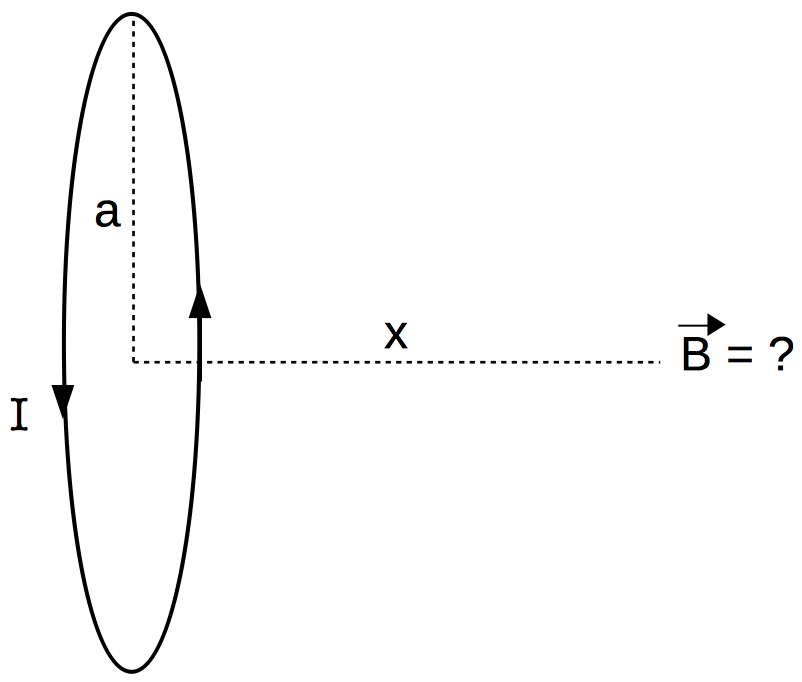
\includegraphics[scale=0.40]{figures/biot-savart/current-loop.png}
\end{figure}

If you consider the radius vectors connecting each small segment of the loop to the point of the field measurment, then a cone is formed.
Furthermore, according to the Biot-Savart Law, $d \vec{B} = \frac{\mu_0}{4 \pi} \frac{I d \vec{s} \times \hat{r}}{r^2}$, the fields produced by each small segment of the loop also form a second cone.

\begin{figure}[H]
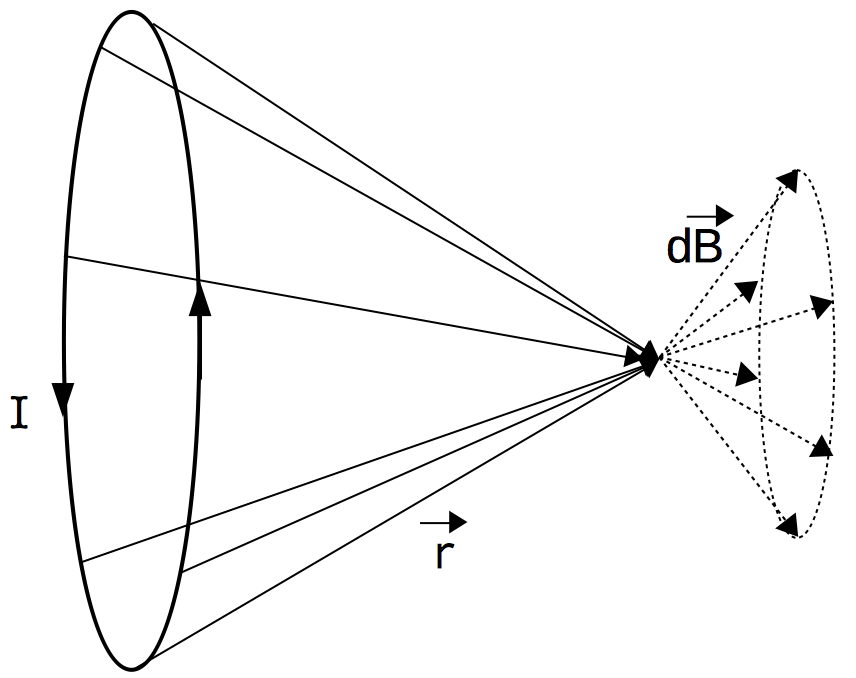
\includegraphics[scale=0.40]{figures/biot-savart/cones.png}
\end{figure}

Construct the two cone system above out of paper using the following technique.
First note that if you cut a straight line from the base of a cone to its tip and unroll the cone, you get a pacman shape (this is very similar to unrolling a cylinder and getting a rectangle).

\begin{figure}[H]
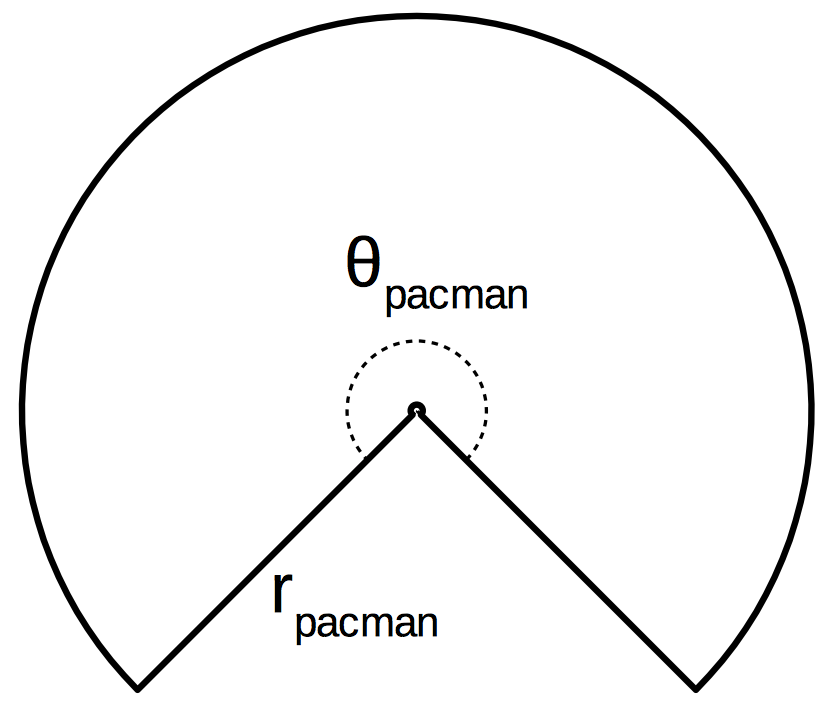
\includegraphics[scale=0.40]{figures/biot-savart/pacman.png}
\end{figure}

Solve for $\theta_{pacman}^{(1)}$, $r_{pacman}^{(1)}$, $\theta_{pacman}^{(2)}$, and $r_{pacman}^{(2)}$ in terms of $a$, $x$, and $h$, where the superscripts refer to the first and second cones and $h$ is the height of the second cone (measured from the center of its base to its tip).
The value of $h$ is arbitrary, it depends on how long you want the field lines to be.
For this lab, let $a = 4.6 \ cm$, $x = 6.3 \ cm$, and $h = 4.8 \ cm$.

\vspace{\baselineskip}

Once you've solved for $\theta_{pacman}^{(1)}$, $r_{pacman}^{(1)}$, $\theta_{pacman}^{(2)}$, and $r_{pacman}^{(2)}$, use a protractor and compass to draw the pacmen on paper, and cut them out.
Tape the pieces together and draw a few relevant vectors on the cones.
If you did everything correctly, the two cones should form $90^\circ$ angles with each other.

\begin{figure}[H]
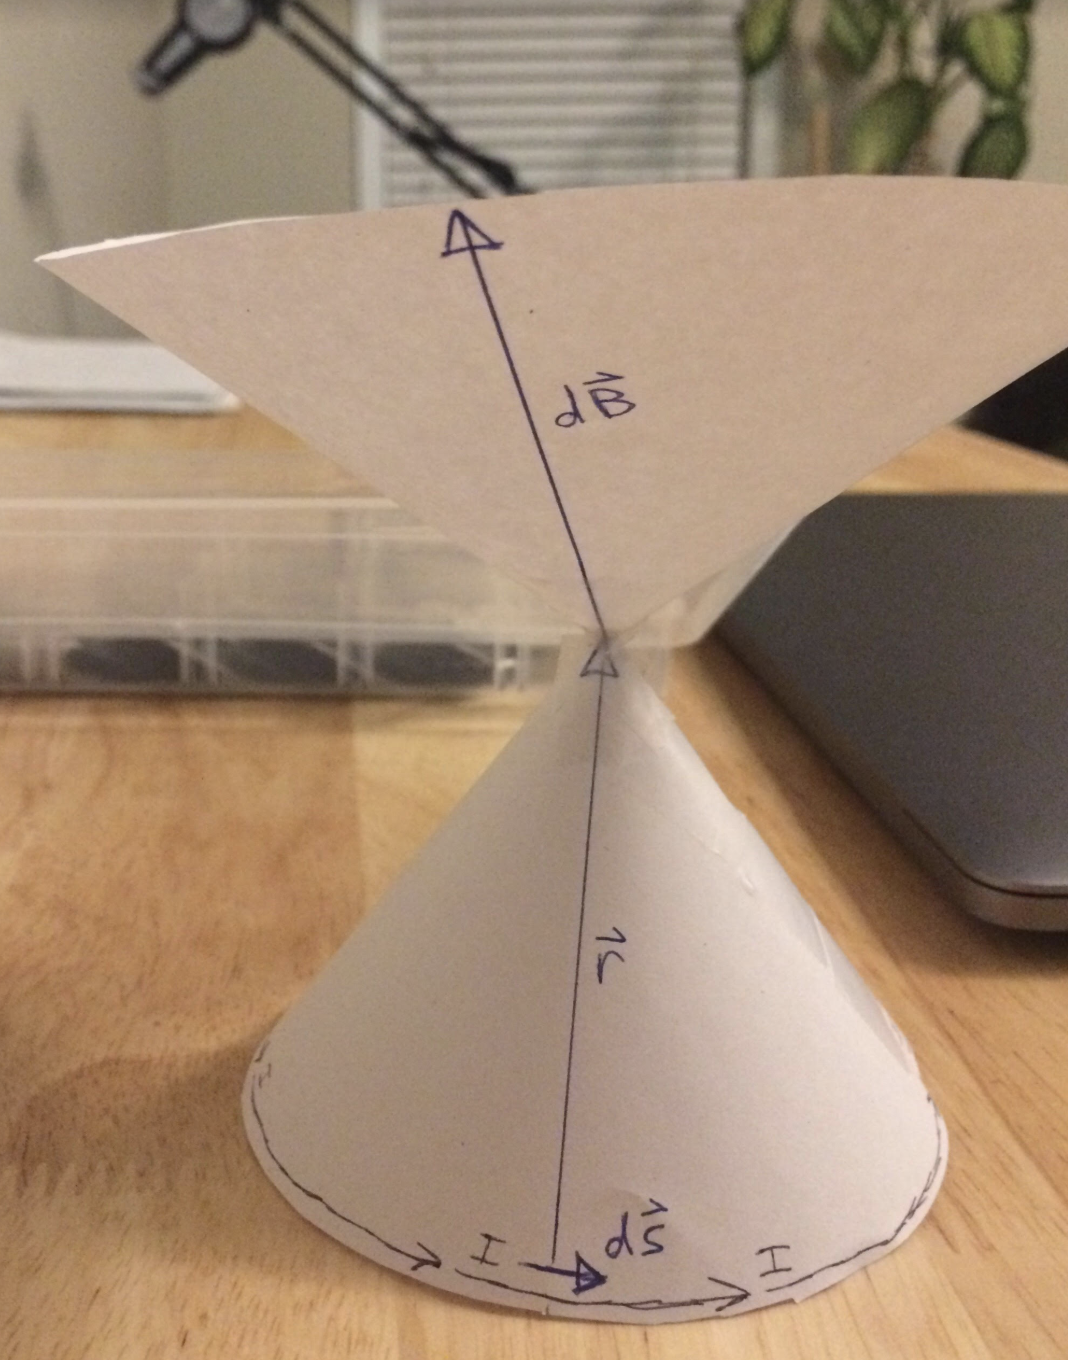
\includegraphics[scale=0.35]{figures/biot-savart/photo.png}
\end{figure}

\pagebreak \clearpage
